\begin{center}

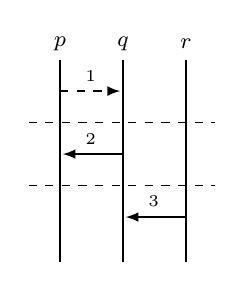
\begin{tikzpicture}[>=stealth,node distance=3.4cm,shorten >=1pt,
    every state/.style={text=black, scale =0.7}, semithick,
    font={\fontsize{8pt}{12}\selectfont}, scale = 0.8]

% \draw (1, -4.25) node{\textbf{(b)}};
%  \node at (-9, -4.25) {\textbf{(a)}};

  %MACHINES
  \draw (0,0) node{$p$} ;
  \draw (1,0) node{$q$} ;
  \draw (2,0) node{$r$} ;
  \draw (0,-0.25) -- (0,-3.5) ;
  \draw (1,-0.25) -- (1,-3.5);
  \draw (2, -0.25) -- (2, -3.5) ;
  %MESSAGES
  \draw[>=latex,->, dashed] (0,-0.75) -- (1, -0.75) node[midway,above]{$\amessage_1$};

  \draw[>=latex,->] (1, -1.75) -- (0, -1.75) node[midway, above] {$\amessage_2$};
  %\draw (0.5,-1.7) node{$\cdots$};
  %\draw[>=latex,->] (1, -2.25) -- (0, -2.25) node[midway, above] {$\amessage_2$};

  \draw[>=latex,->] (2,-2.75) -- (1,-2.75) node[midway, above] {$\amessage_3$};
%\end{scope}
  \draw[dashed] (-0.5,-1.25) -- (2.5,-1.25) ;
  \draw[dashed] (-0.5,-2.25) -- (2.5,-2.25) ;


\end{tikzpicture}
\captionof{figure}{MSC $\msc_3$}
\label{fig:msc_weak_S_exist}

\end{center}
